      \subsection{Nástroje pro replikaci v PostgreSQL}

      PostgreSQL nabízí hned několik nástrojů pro replikaci. Je možno použít zabudovanou streaming replikaci, která je dostupná od verze PostgreSQL 9.0, nebo některou z extenzí, například Slony-I, pgpool, Londiste, Bucardo nebo Postgres-XC, pro jejichž srovnání \vizTabulka{tSrovnaniReplikace}. Tato kapitola se dále bude zabývat nativní streaming replikací a extenzemi Slony-I a pgpool.

        \begin{table}[H]
          \caption{Srovnání různých typů dostupných replikačních řešení}
          \label{tSrovnaniReplikace}
          \begin{footnotesize}
            \begin{center}
              \rowcolors{1}{white}{lightgray}
              \begin{tabular}{|c|cccccc|}
                \hline
                {\bf \color{purpurova7}nástroje}	& {\bf \color{purpurova7}typ} & {\bf \color{purpurova7}technika} & {\bf \color{purpurova7}M/M} & {\bf \color{purpurova7}M/S} & {\bf \color{purpurova7}sync} & {\bf \color{purpurova7}async} \\
                \hline
                PostgreSQL 9.3* & fyzická & xlog     & ne  & ano & ano & ano \\ 
                      pgpool-II & logická & proxy    & ano & ne  & ano & ne  \\
                        slony-I & logická & triggers & ne  & ano & ne  & ano \\ 
                       Londiste & logická & triggers & ne  & ano & ne  & ano \\ 
                        Bucardo & logická & triggers & ano & ano & ne  & ano \\ 
                    Postgres-XC & cluster & -        & ano & ne  & ne  & ano \\ 
                \hline
                \multicolumn{3}{l}{\scriptsize{*streaming replikace}} & \multicolumn{4}{r}{\scriptsize{zdroj: Tomáš Vondra, 2011}}\\
              \end{tabular}
            \end{center}
          \end{footnotesize}
        \end{table}

      \subsubsection{Slony-I}
      \label{kSlony}

      Jak píší \cite{Boszormenyi2013} je Slony-I jeden z nejrozšířenějších externích nástrojů pro replikaci PostgreSQL databází. Zároveň se také řadí mezi nejstarší, plně používán je v PostgreSQL již od verze 7.3. a je velmi dobře podporován i dalšími externími řešeními pro PostgreSQL, například programem PgAdmin3, který nabízí správu dat pomocí grafického rozhraní \citep{Boszormenyi2013}.

      Jedná se o {\it trigger-based} replikaci, což znamená, že je ke každé tabulce vybrané pro replikaci přidán trigger, který zajistí replikaci každé změny, která v tabulce nastane. Z toho také vyplývá, že se jedná o logickou replikaci, kdy je možné replikovat pouze změny v datech, tedy tzv. DML\footnote{Data Manipulation Language} příkazy (INSERT, UPDATE, DELETE), nikoli změny struktury databáze, tedy tzv. DDL\footnote{Data Definition Language} příkazy (CREATE, ALTER, DROP). Každá změna struktury se tedy musí provést ručně, což se může jevit jako nevýhodné. Nese to ale i své klady, například možnost výběru pouze některých tabulek. Uživatel vytváří tzv. {\it replikační set}, do kterého se zapíší pouze ty tabulky, které je potřeba replikovat. 

Další výhodou, a to zvlášť v porování se streaming replikací, je možnost replikace dat mezi různými verzemi PostgreSQL bez ohledu na platformu a architekturu. Naopak spíše za nevýhodu je považováno, že si vytváři ke každé tabulce vlastní schéma, do kterého se ukládají replikovaná data, což způsobuje redundanci dat. 

  Slony-I umožňuje multimaster i master-slave replikaci, která je z principu asynchronní. 
  Slony-I replikaci je možno nastavit jako kaskádovou i jako Hot Standby, což
  znamená, že v případě pádu master serveru je slave automaticky povýšen na
  master. Slony-I má vlastní konfigurační nástroj a samotná replikace funguje
  díky vlastnímu replikačnímu démonu, který běží stále, registruje změny a
  kopíruje je na slave servery.

  \subsubsection{Streaming replikace}
  \label{kStreamingTeorie}

  Streaming replikace je nativní řešení PostgreSQL implementované od verze
  9.0. Jedná se o fyzickou replikaci, proto je nutné použití stejné verze
  PostgreSQL, stejné platformy i architektury na všech uzlech replikačního
  clusteru. 
  
  Jde se o {\it log-shipping} replikaci, což znamená, že jsou na slave servery
  posílány záznamy transakčního logu, v PostgreSQL nazývané WAL (Write Ahead
  Log). Do něj jsou změny nejdříve zaznamenávány přímým zápisem na disk a až
  poté potvzeny jako úspěšné. Tento způsob zajišťuje datům naprosté bezpečí,
  protože kdyby došlo k chybě a změny se nezapisovaly na disk, ale pouze do
  cache, mohlo by dojít k jejich ztrátě. Existuje pouze jeden transakční log
  pro jednu instalaci PostgreSQL, proto se replikují vždy všechny databáze a
  není možné výběru jen několika tabulek, tak jako u Slony-I \citep{Boszormenyi2013}. 
 
  Výhodou tohoto nativního řešení je větší efektivita a stabilita replikace,
  než nabízí jiná diskutovaná řešení. Použití toho způsobu replikace však má i
  tu nevýhodu, že aktualizaci databázového systému, operačního systému i
  architektury je třeba provést vždy na všech serverech zároveň.

  Streaming replikace umožňuje pouze master-slave replikaci ve variantách
  synchronní, asynchronní a kaskádová\footnote{podporovaná od verze PostgreSQL
  9.2} a Hot Standby mód.

      \subsubsection{pgpool}
      \label{kpgpool}

Nástroj pgpool, který je stejně jako Slony-I extenzí pro PostgreSQL, je dalším
z nástrojů, který je možno použít pro replikaci dat. Umožňuje však i další
pokročilé funkce jakými jsou sdílení spojení klienta s databází mezi servery
(angl. connection pooling), paralelní uložení dat (angl. parallel query) a
rozložení zátěže mezi více servery (angl. load balancing). 

Nástroj pgpool umožňuje sdílení spojení klienta s databází, což v praxi
znamená, že se vytvoří několik spojení se serverem, která i po skončení dotazu
zůstanou otevřená a připravená pro další použití. Nemusí se tedy navazovat
spojení při každém požadavku ze strany klienta, což velice zrychlí provoz a
zajistí plynulost užívání databáze. Je vhodným nástrojem pro správu velkých
tabulek díky distribuovanému způsobu ukládání dat \citep{pgpool2014}. 

Zároveň pgpool umožňuje rozložení zátěže mezi více serverů v replikačním
clusteru, aby nedocházelo k přetížení jednotlivých uzlů a celkově se zvýšila
rychlost a~efektivita práce s databází. V tomto se pgpool stává prostředníkem
pro komunikaci mezi klientem a serverem. 

Aby nebylo potřeba dát každému
uživateli přístup k jinému slave serveru, nebo přístupy do databáze manuálně
rozkládat skrze složité programové řešení, nabízí se možnost použití pgpool. 
Ten se navenek jeví jako jakákoliv jiný databázový server, do kterého se
uživatelé připojí a  pgpool pak sám rozdělí dotazy mezi uzly v replikačním
clusteru dle aktuální zátěže \citep{Boszormenyi2013}. Zároveň, pokud má
uživatel práva ke čtení i k zápisu, umí na základě aktuálního SQL příkazu
rozhodnout, zda jej přepošle master nebo slave serveru \odkazObrazek{opgpool}. 

Na základě vybraných funkcí je možno použít jeden ze čtyř základních módů, které pgpool poskytuje\footnote{kompletní přehled na \url{http://www.pgpool.net/docs/latest/pgpool-en.html\#config}}: základní, replikační, master/slave a paralelní. V návrh databázového řešení byl použit mód master/slave, který je dále popisován v kapitole \odkazKapitola{kpgpool}.

      \begin{figure}[H]
        \centering
        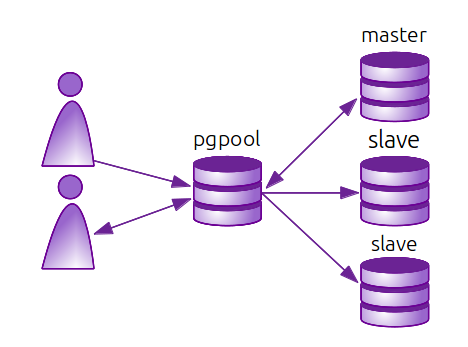
\includegraphics[scale=1]{../../../grafy/obr/schema_pgpool.png}
        \caption{Zjednodušené schéma pgpool v módu master/slave}
        \label{opgpool}
      \end{figure}

